%
%
%
\clearpage
\section{Characterization of electromagnetic shower properties with
a sampling calorimeter}
\label{sec:emshowerproperties}

\FIXME{Add introduction}

%%
%%
%%
\subsection{Longitudinal evolution and energy estimation}
\label{subsec:longevol}

Figure~\ref{fig:showerfits} shows the longitudinal shower evolution
for single electron events as function of the \Xnot transversed in the
detector.

\begin{figure}[h!]
  \begin{center}
    \caption{From {\em left} to {\em right}: energy deposits in different Si layers for single
      electron events with energies: 10, 25, 50, 100\GeV. The deposits
    are shown as function of the transversed distance in \Xnot
    units. A fit is overlaid using the function form described in the
    text. The results obtained for the different energy estimators considered in the analysis
    are shown in the caption}
    \label{fig:showerfits}
  \end{center}
\end{figure}


Different methods are used to estimate the total energy of the shower:

\begin{description}

\item[Raw energy] we sum inclusively of all the energy deposited in
  the Si layers assuming the full sensitive area volume;

\item[Weighted energy] we sum the energy deposited in each Si layer
  normalized by the material overburden of the sampling section,\ie:

\begin{equation}
{\rm weighted~E}=\sum_{i=1}^{N} \frac{X_0^i}{X_0^1}\cdot E_i
\label{eq:weightenest}
\end{equation}

For the baseline setup these weights correspond to 1 for section A,
1.6 for section B and 2.4 for section B.
These weights can also be optimised to minimise the energy resolution
for the incoming energy range of interest.

\item[Shower profile fit] - a functional form is used to adjust the
  measured energy deposits in each layer:

\begin{equation}
\mathcal{E}(x)=\alpha\cdot x^{a} \cdot e^{-bx} 
\label{eq:showerprof}
\end{equation}

where x is the transversed material overburden measured in \Xnot
units. This approach is expected to recover the shower leakage for
higher incident energies.

\item[Shower maximum] - the position of the shower max can be used as a
  coarse estimator for the energy. It can be estimated after the
  shower fit by the ratio $X_{0}^{\max}=b/a$.

\item[Hit counting] - this estimator, altough impossible to be used in
  reality, is used to gauge to potential of the setup. We use the
  weighted sum  of the number of hits generated per Si layer as an
  estimator of the initial energy. The weights are the same as define
  in Eq.~\ref{eq:weightenest}.

\end{description}

For the first two methods, the total energy is fitted, per incoming
energy generated, by a gaussian. The mean is used for calibration, and
the resolution is defined as the ratio of the width over the mean.

Using single electron events we obtain
the calibration curve shown in Fig.~\ref{fig:baselinelinandresol}
{\em left}. Figure~\ref{fig:baselinelinandresol} {\em right} shows the energy
resolution as a function of the incoming energy. For incoming energies
below 150\GeV, 2500 events have been generated. For higher energies
1250 events are used.

\begin{figure}[h!]
  \begin{center}
   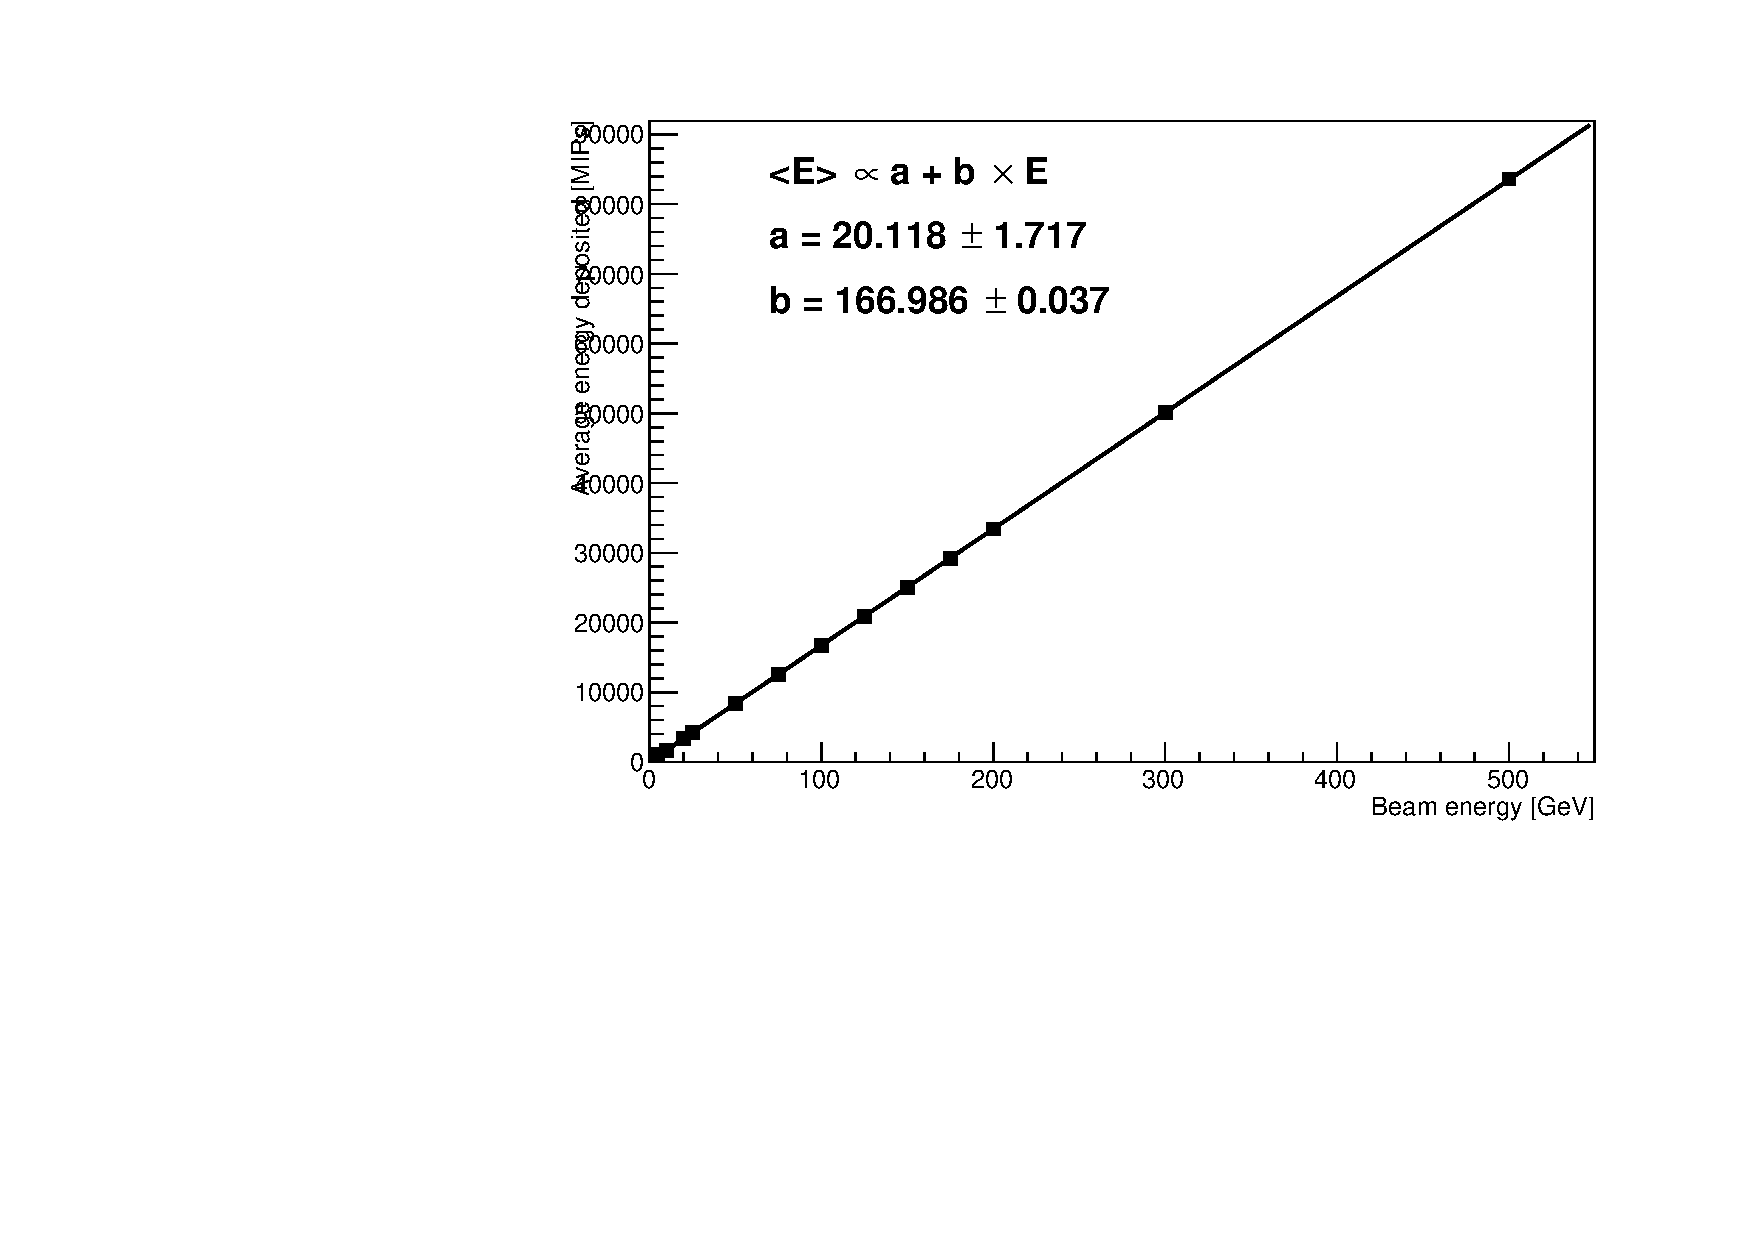
\includegraphics[width=0.48\textwidth]{figures/e_calibFit.pdf}
    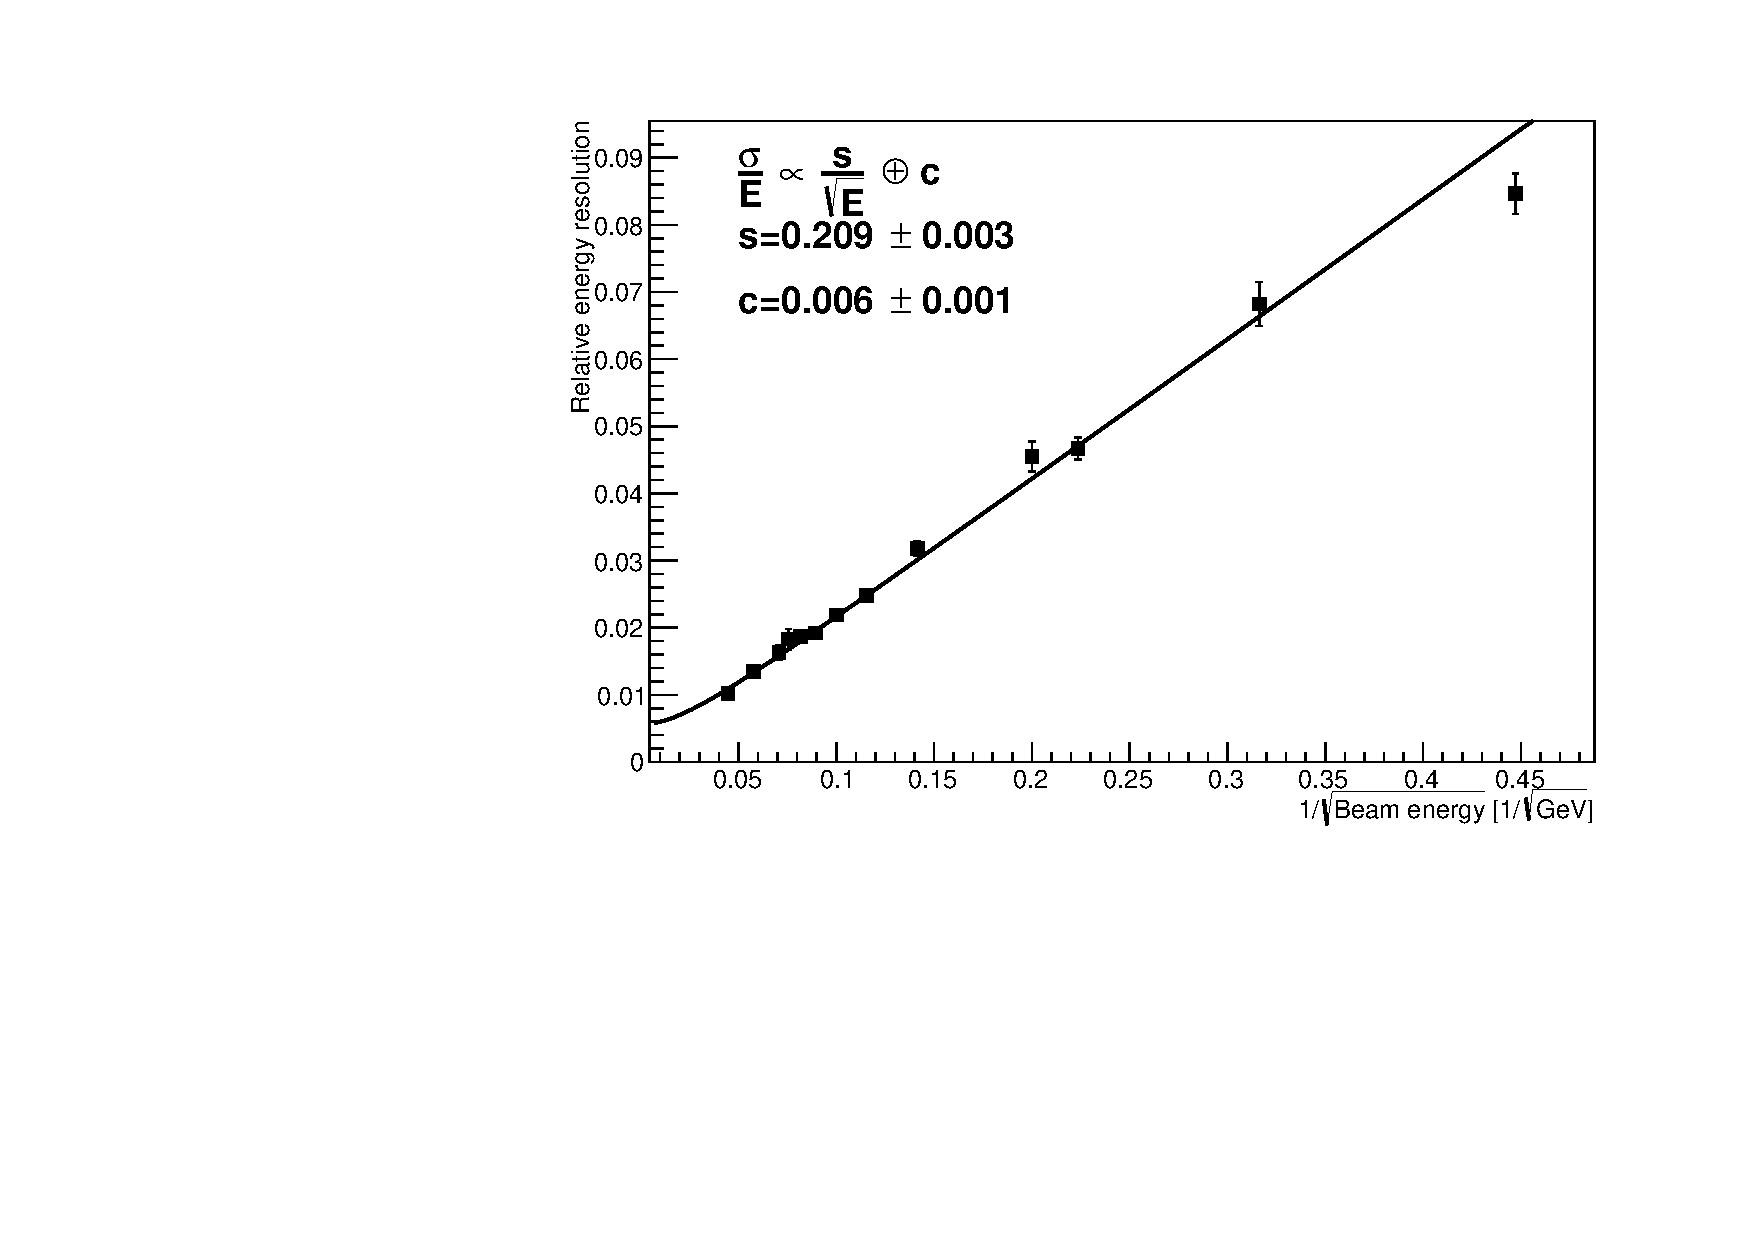
\includegraphics[width=0.48\textwidth]{figures/e_resoFit.pdf}
    \caption{{\em Left}: reconstructed energy (in MIP units) as a function of the generated
      energy E. {\em Right}: energy resolution as a function of
      $\frac{1}{\sqrt{E}}$. In both cases single electron events are simulated.}
    \label{fig:baselinelinandresol}
  \end{center}
\end{figure}


%%
%%
%%
\subsection{Transverse shower evolution and shower containment}
\label{subsec:transvevol}

\FIXME{Describe transverse shower properties and Moliere radius}
